\chapter{Introduction}
\label{chapter:introduction}

Nowadays, computers are invading our daily lives, from work to leisure, from fancy smartphones to embedded peacemakers that regulate the heartbeat of people.
As human beings, we are known to use tools to enhance our bodies. Moreover, thanks to computers, we pushed that step even further, to the point where now we are using machines to extend our brains, from equation solvers to tools to recommend to us where we should invest our money, what we should eat, and even who fits best as our partner.
One major aspect of computers that became omnipresent in our lives is the Internet, which is a network of networks that connects millions of computers all over the world. According to Internet World Stats\footnote{\url{https://www.internetworldstats.com/stats.htm}}. The number of people connected to the Internet has increased by 4.4 billion in 2019, reaching 4.54 billion worldwide, or 59.2\% of the world population.

The internet has evolved from a place where government researchers share information in the 60s to a means of Communication at the beginning of the century, and now it is a place where we can find almost anything we want, from information to entertainment, from social media to e-commerce.

At present, a large chunk of the global economy and most governments have shifted their operations to the Internet, at least partially and sometimes wholly; this includes online shops, banking, advertising, video and music consumption, and even public functions.

Moreover, Due to The pandemic caused by COVID-19 disease, the world has been forced to adapt to a new way of living, which has been accelerated by the Internet. The Internet has become a necessity for people to work, study~\cite{naresh2020education}, and even health consultations~\cite{liaw2021primary}.

On the other hand, as humanity, we face a major challenge, which is climate change. The Intergovernmental Panel on Climate Change (IPCC) has warned that the world has only 12 years to limit the global temperature rise to 1.5\degree C and that the world has to reach net-zero emissions by 2050 to avoid the worst effects of climate change. The IPCC has also warned that the world has to reduce its emissions by 45\% by 2030 to reach the 1.5\degree C target~\cite{portner2022climate}.

To survive, we have come up with three solutions,
The first one includes finding a new planet that we can populate and live on\footnote{\url{https://en.wikipedia.org/wiki/Interstellar_(film)}}, which is called the Planetary Migration~\cite{mapstone2022cyanobacteria}.
Meanwhile, the second solution is to provide new sources of energy, such as nuclear energy, wind energy, and even fusion energy~\cite{gross1984fusion}. The third solution is to reduce our emissions, which is the main focus of this thesis.

While there are many fields where one can optimize energy consumption. Our focus is on the Information and Communication Technology (ICT) sector, which is expected to account for around 4\% of global greenhouse gas (GHG) emissions in 2020, with an alarming 8\% growth rate, according to the French think tank The Shift Project\footnote{\url{ https://www.theshiftproject.org/article/ict-environmental-impact/}}.
According to \emph{Statista}, the Energy consumption of ICT increased from 4.3 exajoules in 2018 to 5.8 exajoules in 2025\footnote{\url{https://www.statista.com/statistics/271139/energy-consumption-of-ict-worldwide}}.
\begin{figure}[!h]
    \centering
    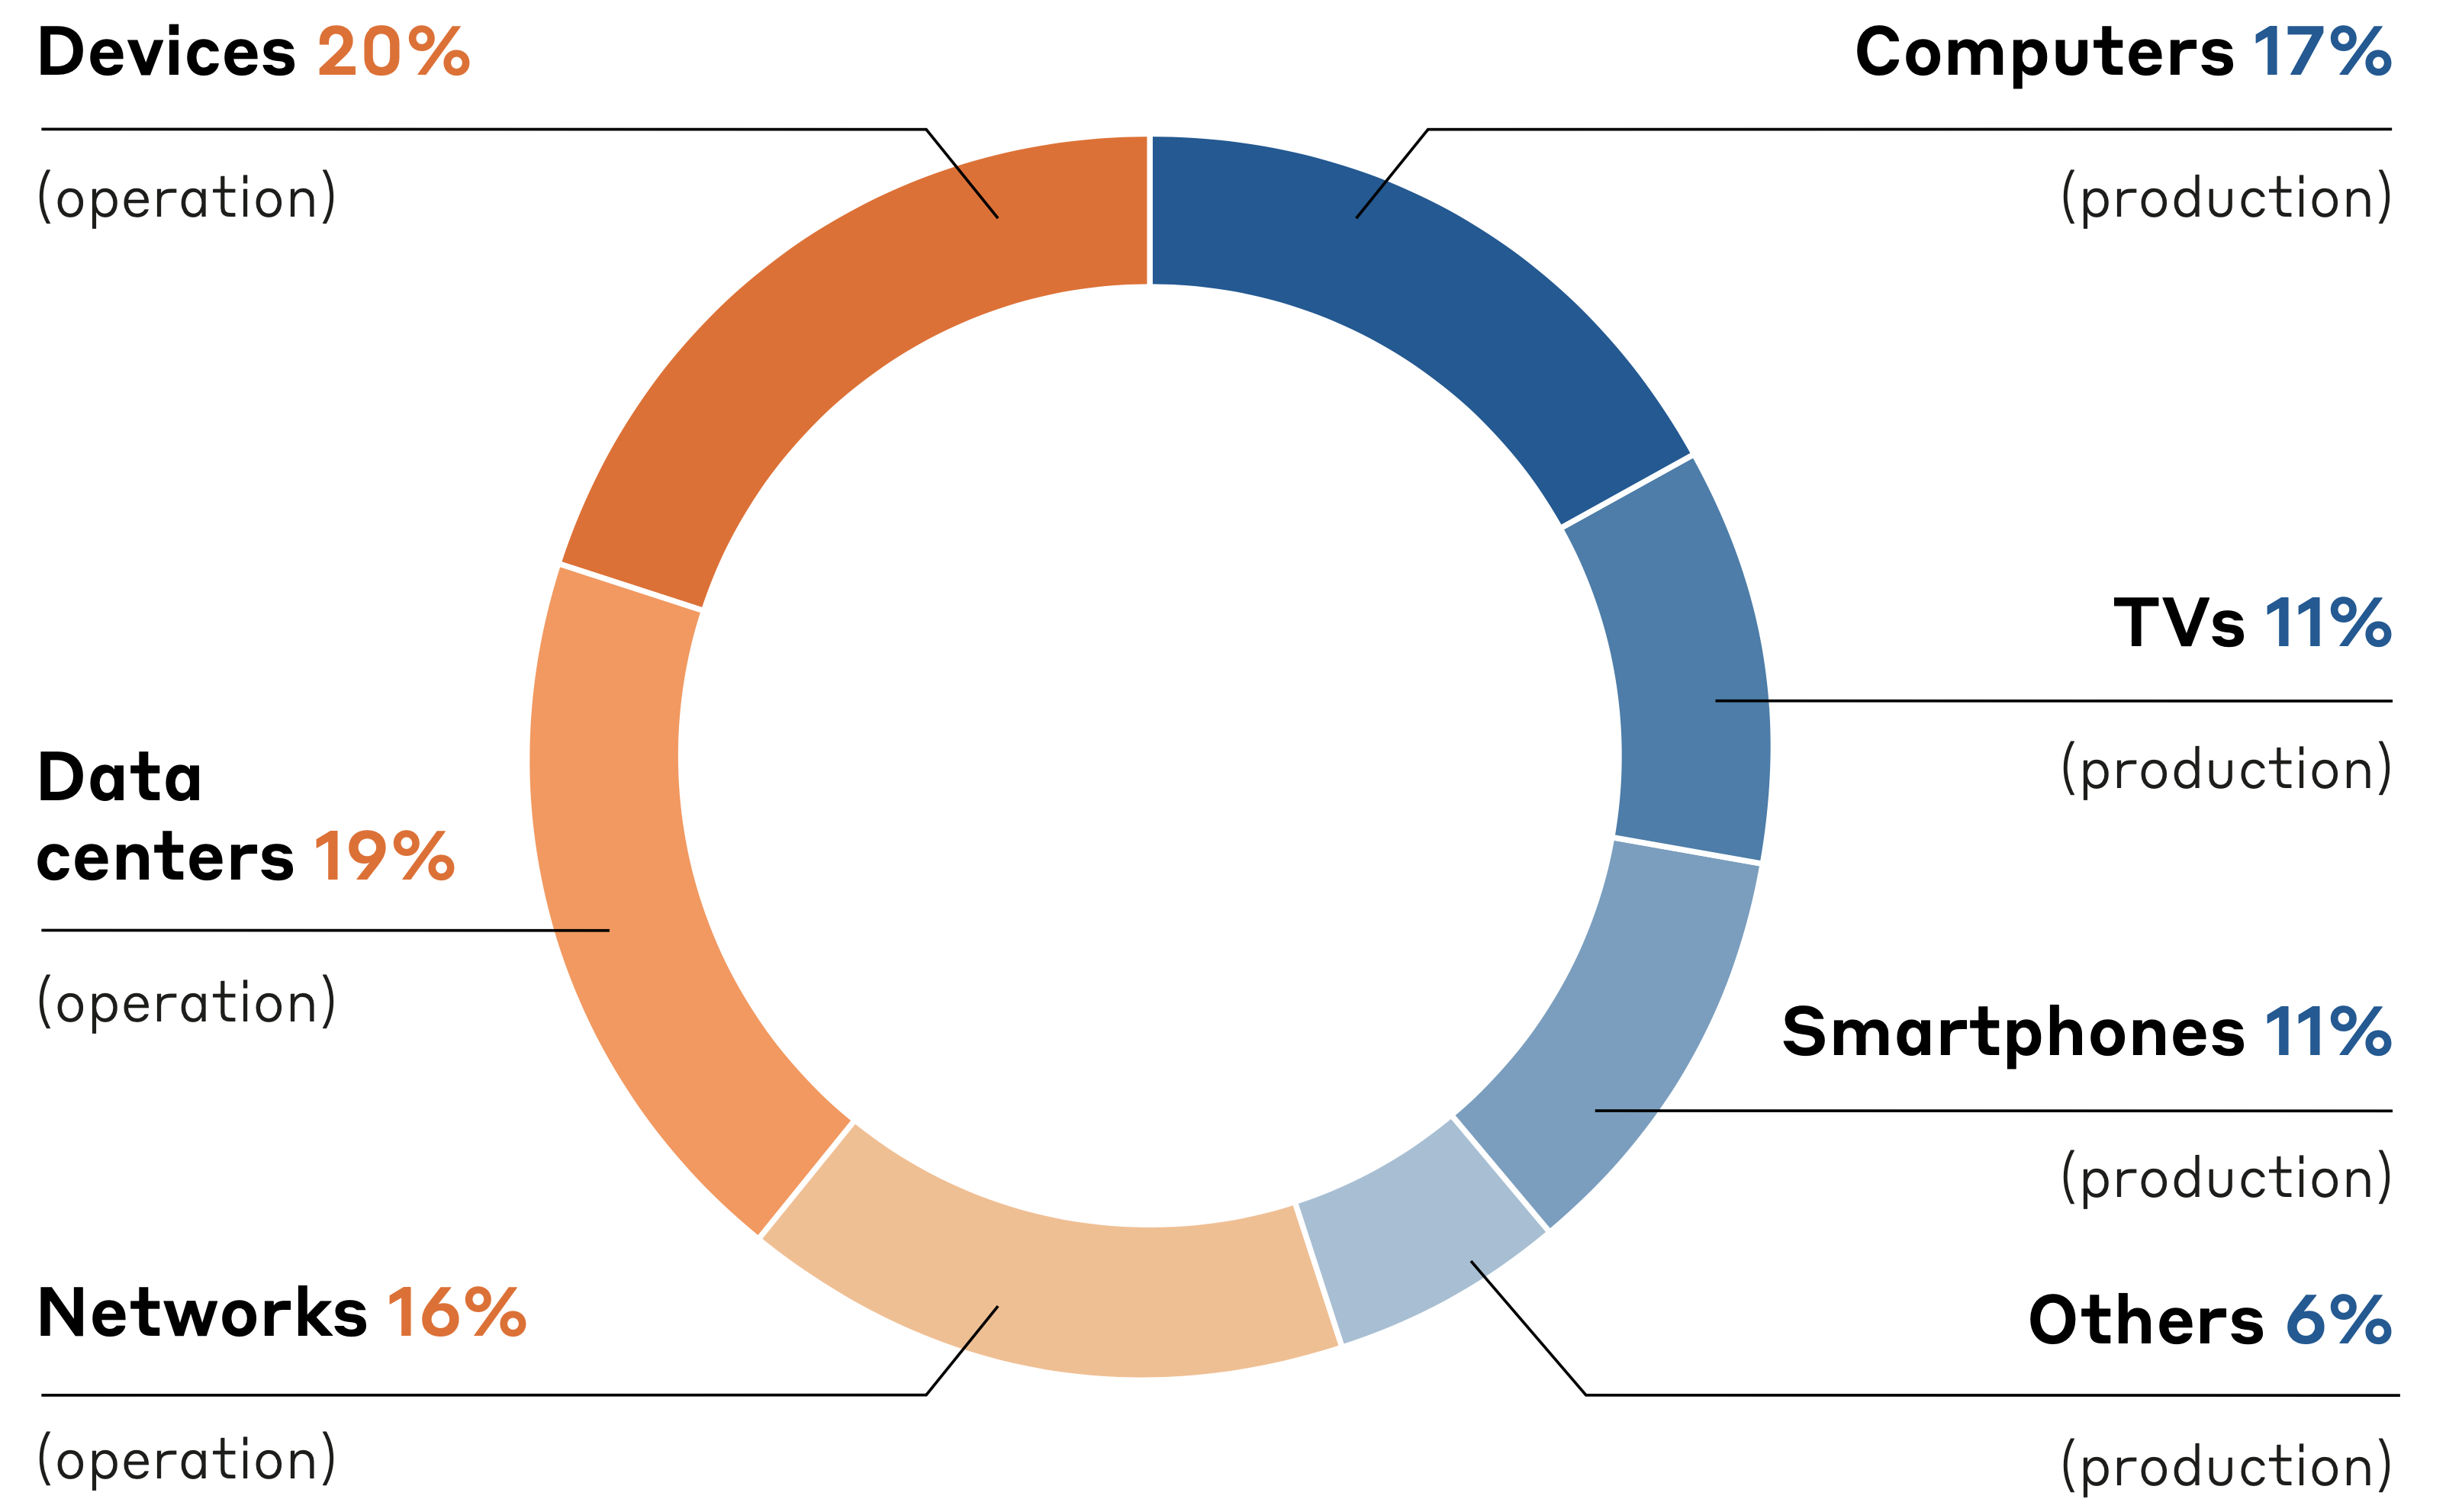
\includegraphics[width=0.8\linewidth]{chapters/distribution_of_ict_consumption.png}
    \caption{Final energy consumption of digital technologies by item in 2017}
    \label{fig:distribution_of_ict_consumption}
\end{figure}

Figure~\ref{fig:distribution_of_ict_consumption} shows the distribution of ICT consumption in 2018, where the largest chunk of the energy consumption is due to data usage, aka 55\% of the energy consumed where 35\% of this energy is used by data centers. Reducing energy consumption means reducing the impact 19\% of the ICT energy consumption has on the environment.

In 2020, the market for data center services was worth 48.9 billion\$. It is thought that this number will go up to 105.6 billion\$ by 2026~\cite{inshakova2022data}. This growth is caused mainly by:
\begin{itemize}
    \item Shift to remote lifestyle: work, education, and entertainment.
    \item Increase in the number of connected devices (IoT)
    \item Development of data-hungry technologies such as Machine learning, AI, Big data, and so on.
    \item Edge computing and 5G.
\end{itemize}

With this increase in the number of data centers comes an increase in energy consumption, which is a major problem for the environment.
in 2018 datacenters consumed around 205 terawatt-hours (TWh)\cite{schneider2021world} which is equivalent to the energy consumption of 1\% of the total world's electricity. This ratio increased up to 1.5 \% in 2020 according to the Journal of Science~\cite{mytton2021data}. Figure~\ref{fig:data_centers_power_distribution}, as one can see, While 40\% of the energy consumed by data centers is used for cooling, another 40\% is used by the servers themselves. Therefore optimizing these two aspects can have a major impact on the energy consumption of data centers.
\begin{figure}[!h]
    \centering
    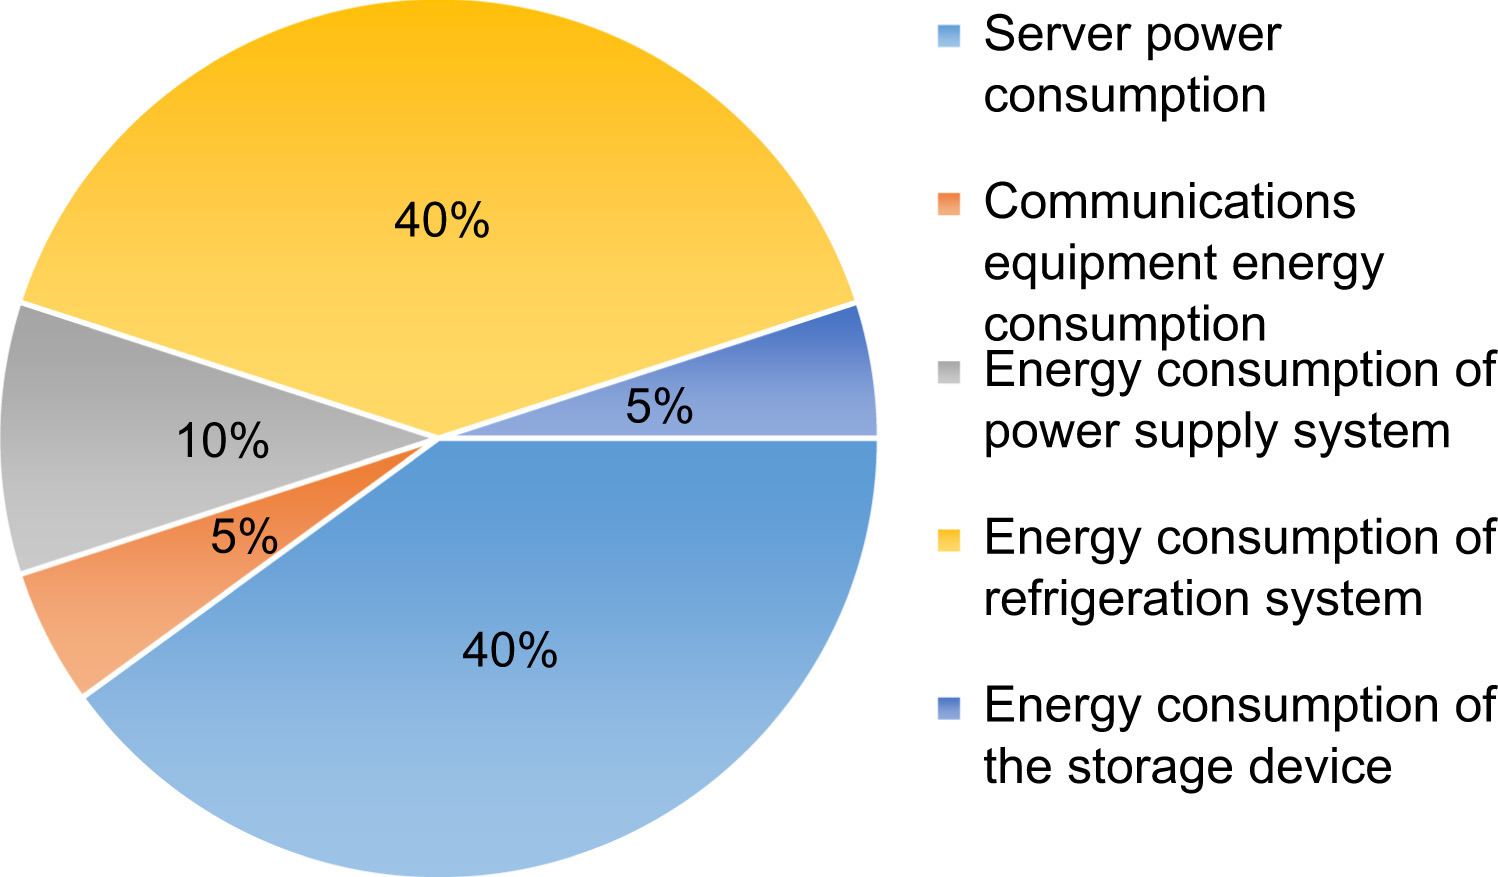
\includegraphics[width=0.6\linewidth]{chapters/data_centers_power_distribution}
    \caption{Distribtuion of power consumption in a data-center\cite{rong2016optimizing}}
    \label{fig:data_centers_power_distribution}
\end{figure}

Researchers are trying to reduce the energy consumption of data centers through different angles. Some of the works are focused on the hardware side, such as using new hardware architectures that are more energy-friendly, such as the use of GPUs instead o ARM processors instead of CPUs~\cite{aroca2012towards}. Others are trying to optimize the cooling system, this can be achieved by using more efficient cooling systems, putting data centers in cold locations or under water~\cite{simon2018project}, or even using the waste heat for other purposes such as heating buildings\cite{bouzel2021distributed,cao2021carbon}.

A third approach is to optimize the software, by making software more energy-efficient. In this thesis, we focus on this approach, and we try to optimize the software by reducing the number of computations that are done by the software.

The best way to do so is to formulate a theory behind the energy consumption of algorithms, such as the complexity and the o notation.
Unfortunately, this is not possible in the current state of the art. Due to the lack of knowledge about the energy consumption of the algorithms, and the strong correlation between this consumption and the hardware configuration.
Unlike algorithm optimization in the field of performance, which is agnostic toward the platform, the energy consumption of the algorithms is dependent on the execution environment.
Therefore, for the moment we will start by formulating some hypotheses and explore them using empirical analysis.
Figure~\ref{fig:thesis_position} highlights this thesis's position on the sustainability of ICT\@; while this thesis only addresses a small portion of ICT's energy usage, we feel it is a step in the right direction for additional solutions to mature in order to preserve humanity.

\begin{figure}[!h]
    \caption{Our position in the IT sustainability research}
    \label{fig:thesis_position}
    \centering
    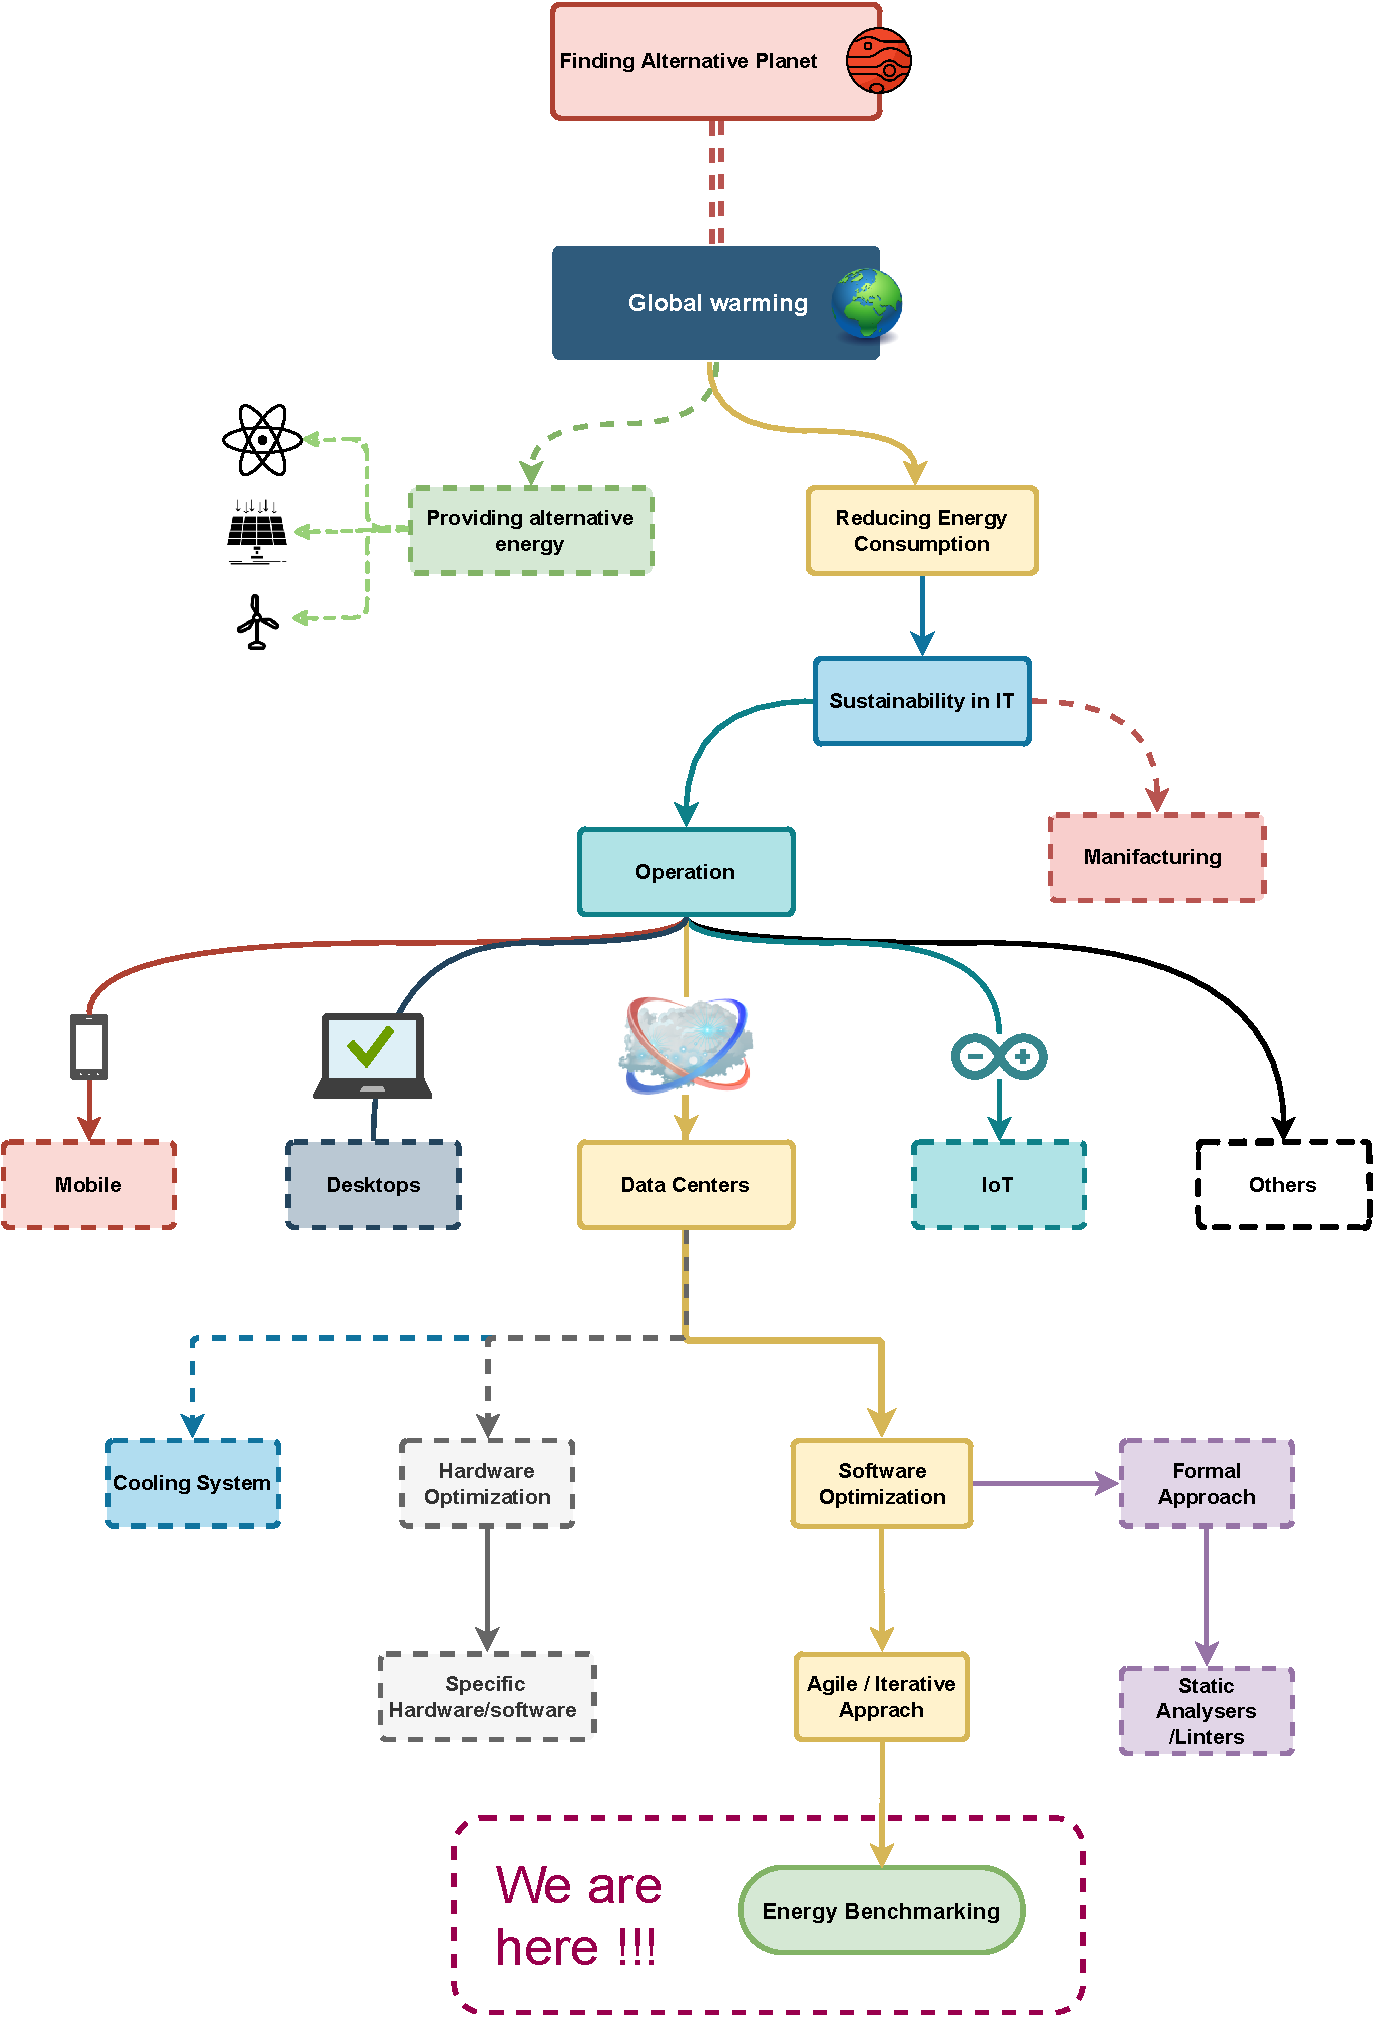
\includegraphics[width=0.8\textwidth,height=\textheight,keepaspectratio]{chapters/thesis_position.pdf}
\end{figure}
\subsection{Objectives}
The purpose of this thesis is to help developers build more energy-efficient software. Unfortunately, when it comes to the energy consumption of programs, there is a lack of awareness and knowledge among software developers~\cite{ournani2020reducing,pang2015programmers,pinto2014mining}. This is mainly due to the lack of tools that can help developers understand the energy consumption of their programs. Therefore we aim, to provide clear, understandable, and easy-to-use tools and guidelines that can help developers reduce the energy consumption of their programs.

In order to reduce the energy consumption of software, we can use three strategies.
The first one consists of \emph{reducing energy consumption by reducing the execution time of the program}. The most intuitive way for developers, as the optimization of software's performance, is a key metric for most programs. There fore in this case, reducing the energy consumption of software is just a happy side effect of optimizing the performance of the software.


The second strategy is \emph{optimizing the energy while trying to keep performance}. In this strategy, we aim to reduce the energy consumption of software without impacting its performance of the software. This is a more challenging task, as it requires a deeper understanding of the software's energy consumption. The main focus of this thesis is to provide tools and guidelines that can help developers in this task.


The final strategy consists of \emph{deleberately reducing the performance of the software in order to reduce its energy consumption}. The goal of this method is to reduce energy usage by sacrificing execution time. This strategy is useful while dealing with services since the task has an unlimited execution time. The second part is to use some. opportunistic schedulers, which will stop the software if it is estimated to spend more energy. This strategy will be discussed first in Chapter~\ref{chapter:porgramming_langauges}, then we will continue with this strategy in the perspectives section.



\subsection{Organization}
\begin{figure}[!h]
    \centering
    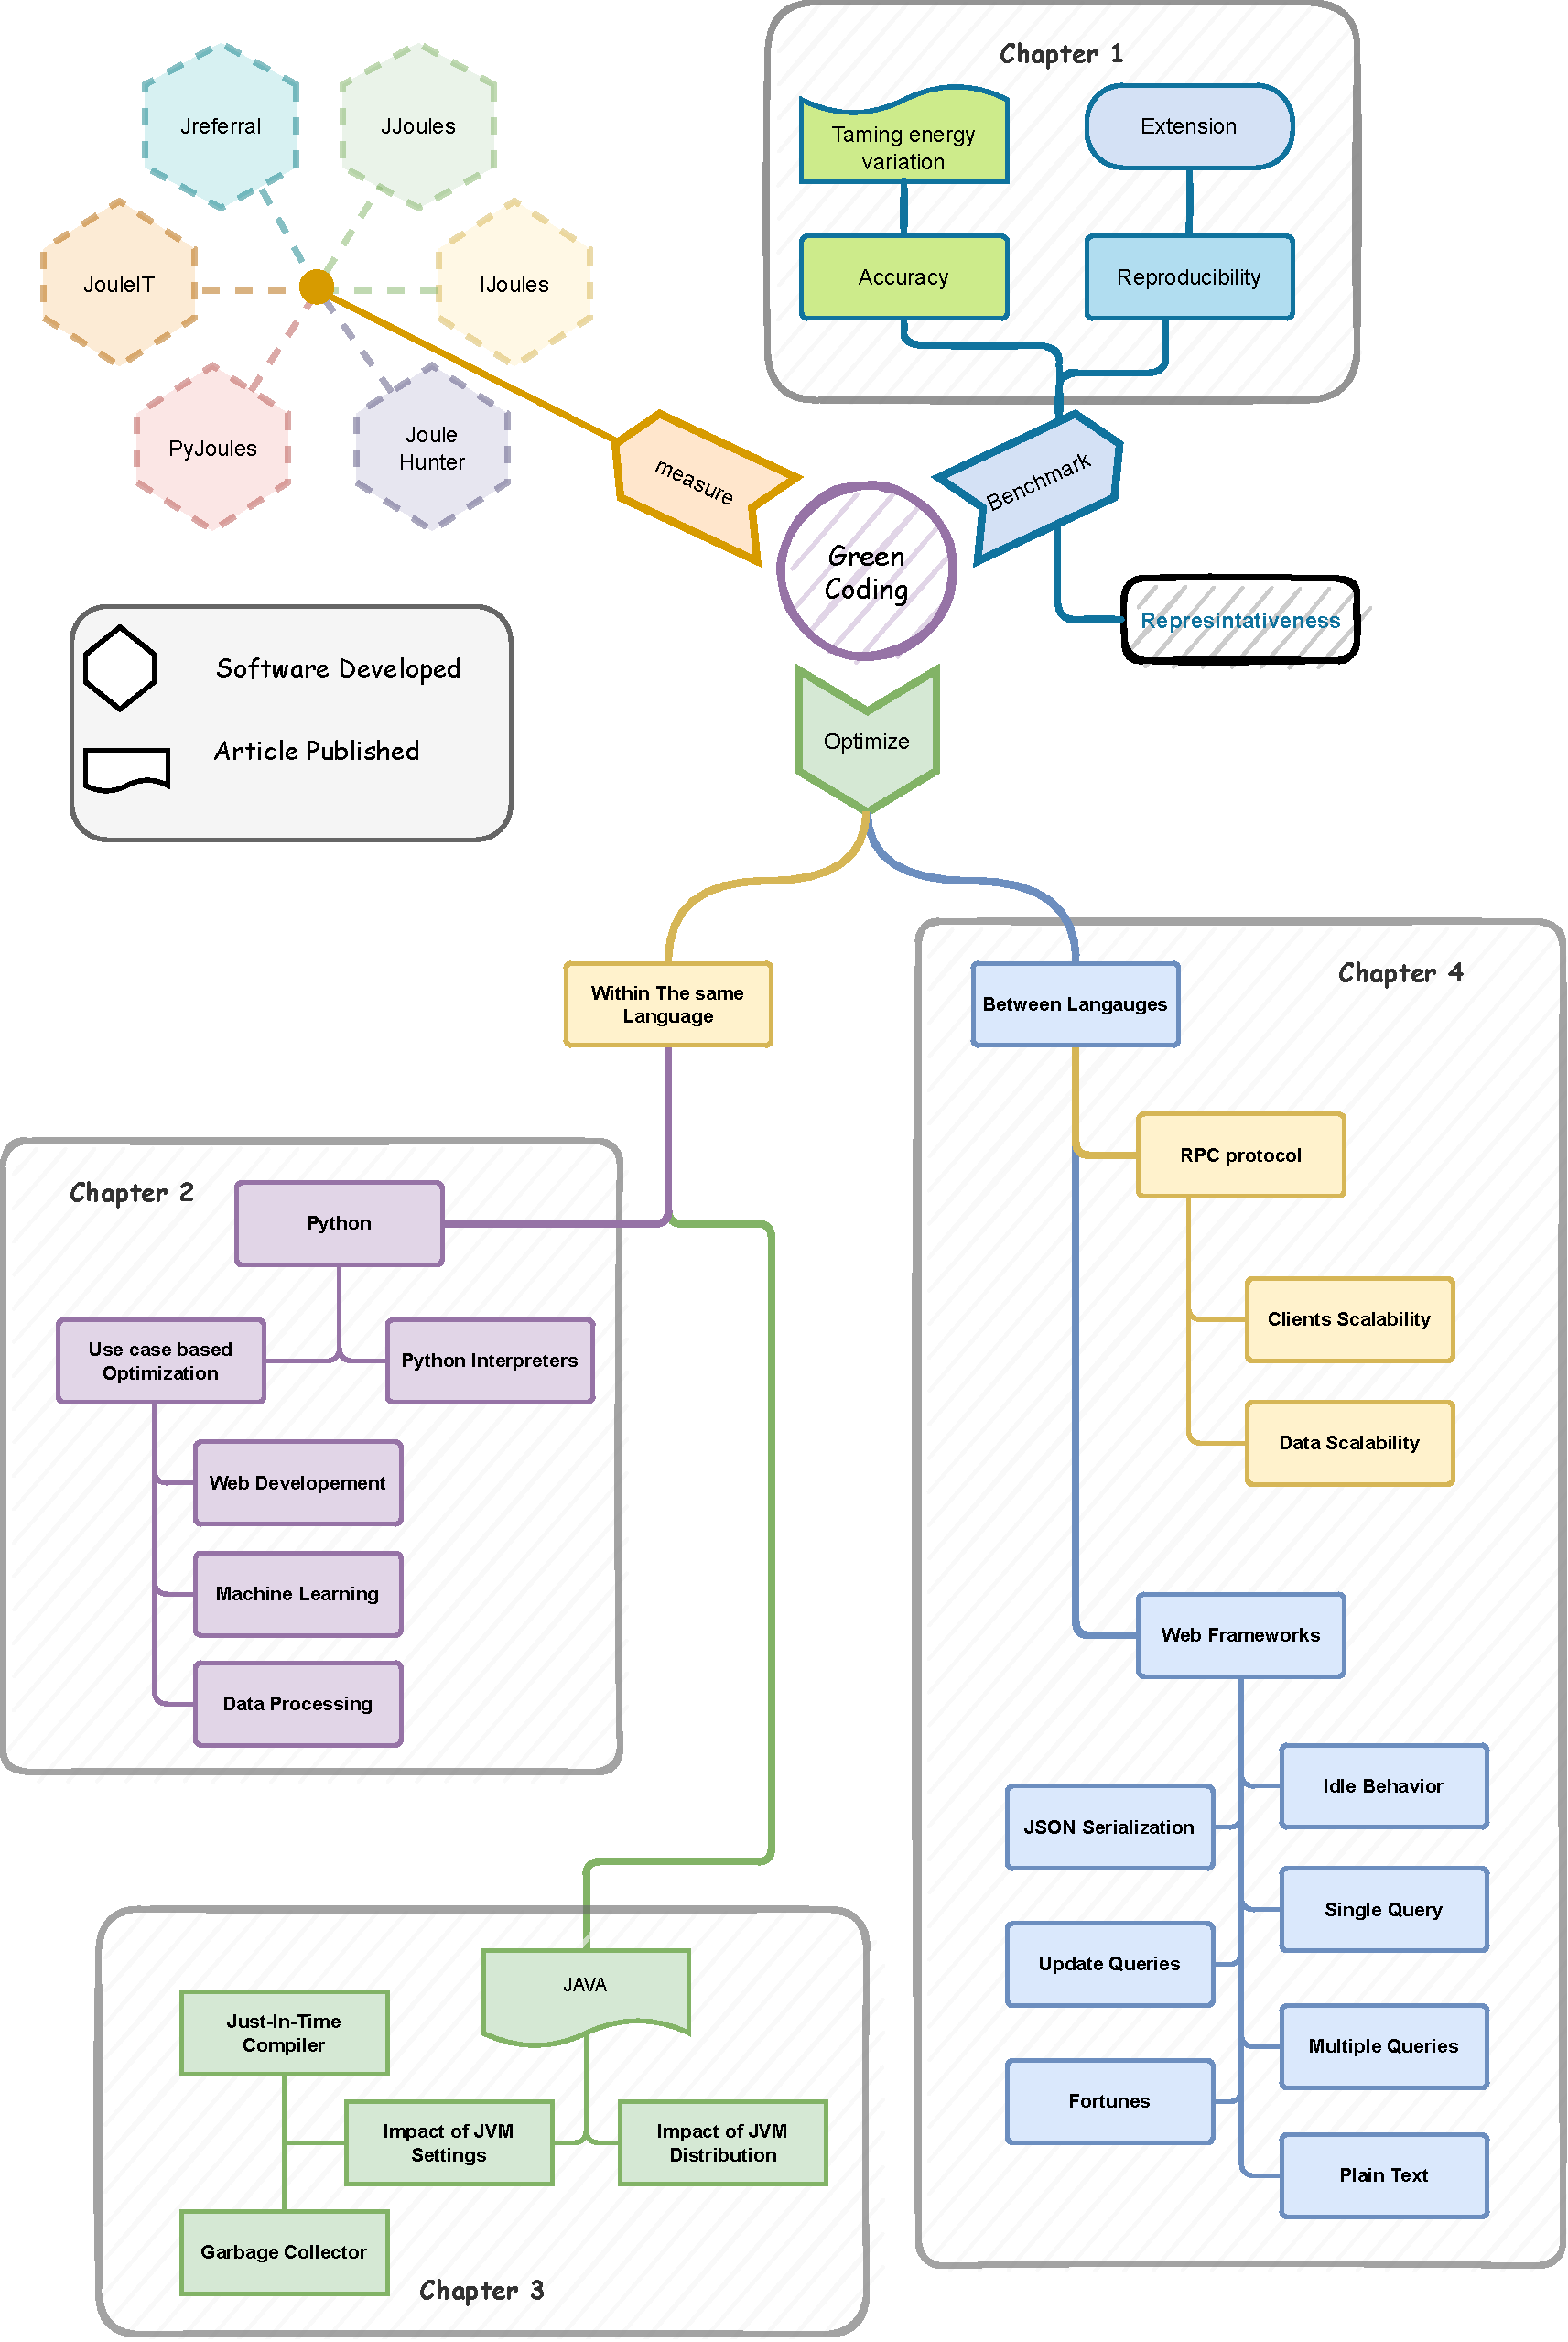
\includegraphics[width=0.8\textwidth,height=\textheight,keepaspectratio]{chapters/thesis_contributions.pdf}
    \caption{Contributions done during this thesis }
    \label{fig:thesis_contributions}
\end{figure}

Figure~\ref{fig:thesis_contributions} summarizes the work completed for this thesis As mentioned in the previous section, our goal is to help developers reduce the energy consumption of their programs during execution.
We will use an empirical approach to accomplish this. As a result, we will require some tools to assist us in this task. To begin, we will provide a tool to assist developers in measuring the energy consumption of their programs. The rest of the document is outlined below.

\begin{itemize}
    \item \cref{chapter:literature_review} provides a literature review of the energy consumption of software. First, it introduces the challenges that one can encounter when running an empirical study, \emph{reproducibiliy}, \emph{accuracy}, and \emph{representativeness}, the ways in the state of the art overcome these challenges in the field of computer sciences. Then, it narrows down to the energy consumption of software and the challenges that one can encounter when measuring the energy consumption of software. In this section, we provide the literature approaches used to measure energy consumption and classify them, compare them and discuss their pros and cons when used for our research. After that, we will tackle the challenge of accuracy within the field of energy consumption, and discuss how the literature tried to overcome these challenges. Finally, we will present some of the most recent works in the field of software energy consumption optimization.
          % We conclude this chapter by providing a simple method that we will use for the rest of the thesis to optimize the energy consumption of software. \textbf{BMO} : benchmark , measure and optimize.  
    \item \cref{chapter:benchmarking} This chapter will discuss two facets of empirical tests and how we adapt them to energy consumption measurements. First, we will discuss the reproducibility challenge and how to overcome it with the usage of containers, then we will push this approach further by proposing and new protocol to make tests not only reproducible but able to be extended with other features to overcome the rapid pace of software evolution. The second part of this chapter will discuss the aspect of accuracy when it comes to energy consumption measurements. This section demonstrates how energy measurements might differ and produce conflicting results for the same work when run on identical machines or even the same machine. Then it will provide some solutions to reduce this energy variation and improve the accuracy of the measurements.
    \item After setting the ground for energy benchmarks in the previous chapter, we start to discuss energy consumption one of the most popular programming languages in the world Python, in \cref{chapter:python}. This chapter starts by presenting how much python costs in terms of energy consumption compared to other languages. then it provides some statistics about its popularity and typical use cases. Then in section \ref{python:sec_insights} we will present the impact of python on energy consumption in three typical use cases, machine learning, web servers, and data manipulation. For each use case, we compare the energy consumption of several approaches and provide guidelines on how to optimize the energy consumption of python programs in these use cases. Finally, we provide a nonintrusive way to optimize energy consumption without altering the code of the program. We will do this by using a different implementation of the python interpreter. This not only allows developers to spend less time optimizing their code but also allows them to use it on the legacy code that they cannot modify.
    \item Motivated by the outcomes of the nonintrusive optimization, we follow this strategy on one of the most popular legacy code base applications programming languages, JAVA. In \cref{chapter:java}, we try to optimize the java code, using by changing the default JVM implementation. We will compare the energy consumption of $12$ benchmarks using $52$ implementation, each benchmark is dedicated to a typical use case. After that, we study two of the JVM features, JIT, AND GC, and show their impact on the energy consumption of the JAVA code.
    \item In contrast, \cref{chapter:porgramming_langauges} will use the flexibility provided by the micro-services architecture~\cite{dmitry2014micro} to analyze each programming language's energy behavior in light of various web scenarios to optimize the energy use of web services. We will first examine the effects of the various programming languages when dealing with the Remote Procedure Call (RPC) Protocol. In this instance, we will use two scaling factors: the number of concurrent clients and the size of the requests. Then we will compare $261$ web frameworks, each implementing the same website using seven use cases. This analysis aims to look at how each technology uses energy in different kinds of web situations.
    \item Finally, we conclude our work in \cref{chapter:conclusion} by summarizing the work done in this thesis and discussing the future work that can be done to further reduce the energy consumption of software.
\end{itemize}

% First, we create a benchmarking protocol that serves researchers and practitioners, experimenting with their approaches and solutions to reduce the energy consumption of programs.
% Then, using this protocol, we analyze and try to optimize the energy consumption of one of the most popular programming languages, Python. We first study python within its most use cases, machine learning, and web Development. Then we try to optimize the energy consumption on the outer side, this can be achieved by targeting the interpreter itself.
% After that, we continue our non-intrusive approach, by targeting the impact of the virtual machine on the JAVA code. This not only helps practitioners improve their software energy without changing their code, but is also beneficial for reducing the energy consumption of the legacy code with almost zero cost.
% Finally, we will shift our focus to other programming languages and compare the energy consumption of different programming languages.
% We consider two main use cases. The RPC protocol, and web servers.

% we have three scenarios, to reduce energy consumption :
% 1. win-win, reducing energy consumption by enhancing the performance: the first one is done by default by most of the developers and performance engineers, which is to optimize the code itself
% 3. win neutral, reducing energy consumption while keeping the same performance: the second one is finding reducing the energy consumption while trying to keep the same performance, which the work of this theses 
% 2. win loose, reducing energy consumption by reducing the performance: optimizing  the energy consumption by sacrificing the performance of the program itself which is what we call  green faas  we will talk about this in the perspective section


% \url{https://www.statista.com/statistics/871513/worldwide-data-created/}
% https://www.iea.org/reports/data-centres-and-data-transmission-networks

% Our work will be presented in the following chapters:
% \begin{enumerate}
%     \item \ref{chapter:literature_review}: Where we discuss the work done on energy consumption and optimization in software engineering
%     \item \ref{chapter: benchmarking}: It will present a set of guidelines and tools to help practitioners measure the energy consumption of their algorithms.
%     \item: it will discuss the behavior of python and the possible ways to tune it in order to reduce the energy consumption
%     \item: will present a study on java programming language and the impact of the JVM choice on the energy consumption
%     \item: we will present the impact of programming languages on the energy consumption of the algorithms especially when it comes to web services.
%     \item: as a perspective, we introduce the impact of parallelism on energy consumption in time-agnostic cases
% \end{enumerate}
% \subsection*{Contributions}


\section{Contributions}
The contributions of this thesis are summarized as follows:
\subsection*{Conferences}
\nobibliography*
\begin{enumerate}
    \item \bibentry{ournani2020taming}
    \item \bibentry{ournani2021evaluating}
\end{enumerate}

\subsection*{Tools}
\begin{itemize}
    \item \bibentry{Belgaid_JouleHunter_an_2021}
    \item \bibentry{Belgaid_JRefferal_Which_JVM_2021}
    \item \bibentry{Belgaid_Jouleit_a_2020}
          % \item \bibentry{Belgaid_Ijoules_Python_library_2020}
    \item \bibentry{Belgaid_Pyjoules_Python_library_2019}
\end{itemize}

% \subsection*{Posters}
% \begin{itemize}
%     \item \emph{PyRAPL\@: Make your python green again}
%           % TODO : ask romain about the date and the name of the event 
% \end{itemize}
\subsection*{Future Work}
\begin{itemize}
    \item Reducing the energy consumption of Python using non-intrusive techniques
    \item Empirical analysis on the energy consumption of different web frameworks
    \item The impact of programming languages on energy consumption of web services (a case study of RPC protocol)
    \item THow do ORMs affect how much energy is used? A case study of Django and Flask
\end{itemize}


\cleardoublepage
